\documentclass[a4paper,twocolumn,11pt]{jarticle}

\usepackage[dvipdfmx]{graphicx}
%
%\setlength{\oddsidemargin}{-7 mm}
%\setlength{\evensidemargin}{0 mm}
%\setlength{\topmargin}{-17 mm}
%\setlength{\textheight}{240 mm}
%\setlength{\textwidth}{170 mm}
%\setlength{\columnsep}{1.5em}
\setlength{\oddsidemargin}{-12 mm}
\setlength{\evensidemargin}{0 mm}
\setlength{\topmargin}{-27 mm}
\setlength{\textheight}{275 mm}
\setlength{\textwidth}{185 mm}
\setlength{\columnsep}{1.5em}
\newcommand{\qed}{\hspace*{\fill} $\Box$ }
%
\makeatletter
\renewcommand{\@maketitle}{%
  \newpage
  \null
  \begin{center}%
  \let \footnote \thanks
    {\LARGE \bf \@title \par}%
    \vskip 10pt
    {\normalsize \@author \par}%
    \vskip 5pt
  \end{center}%
  \par
  \vskip 0.5em 
}
\renewcommand{\section}{\@startsection {section}{1}{\z@}%
{4.0pt plus 6.0pt minus 3.0pt}%
{2.0pt plus 2.0pt minus 2.0pt}{\large\bf }}
\renewcommand{\subsection}{\@startsection{subsection}{2}{\z@}%
{4.0pt plus 4.0pt minus 3.0pt}%
{1.0pt plus 2.0pt minus 1.0pt}{\large\bf }}
\renewcommand{\subsubsection}{\@startsection{subsubsection}{3}{\z@}%
{4.0pt plus 4.0pt minus 3.0pt}%
{1.0pt plus 2.0pt minus 1.0pt}{\large\bf }}
\renewcommand{\paragraph}{\@startsection{paragraph}{4}{\z@}%
{0.0pt plus 1.0pt minus 0.0pt}{2.0pt plus 1.0pt}%
{\normalsize\bf}}
\renewcommand{\subparagraph}{\@startsection{subparagraph}{4}%
{\parindent}{0.0pt plus 1.0pt minus 0.0pt}{2.0pt plus
1.0pt}{\normalsize\bf}}
\renewcommand{\thesection}{\arabic{section}.}
\renewcommand{\thesubsection}{\arabic{section}.\arabic{subsection}.}
\renewcommand{\thesubsubsection}{\arabic{section}.\arabic{subsection}.\arabic{subsubsection}}
\makeatother


%
\title{振動刺激によるアリの行動変化の映像解析に関する研究}
%副題がある場合
%\title{〇〇〇〇に関する研究 \\ {\Large\bf--副題--}}
\author{JB20S079 ホアンバフン
\\ 指導教員:川嶋宏彰教授}
%
\date{}
%
%
%↓索引生成
%\makeindex
%
%

\begin{document}
\maketitle
\newtheorem{thm}{定理}
\newtheorem{df}[thm]{定義}
\newtheorem{lm}[thm]{補題}
\newtheorem{co}[thm]{系}
\newtheorem{pr}[thm]{命題}
\newtheorem{que}[thm]{問題}
\thispagestyle{empty}

\section{はじめに}
アリはさまざまな環境条件下で生息しており,  外部からの刺激に対する適応能力が求めらる. アリの行動を観察し, その行動を解析する既存研究がある[1, 2]ものの,対象個体数が少数,もしくは計測可能範囲が限られるなどの制限がある.そこで本研究では,近年コンピュータビジョン分野で提案されている個体追跡手法を用いるとともに,これまで十分分析が行われていない,振動刺激に対する行動変化の解析に取り組む.
本研究の全体の流れを図1に示す。


\section{振動刺激提示によるアリの行動変化誘発実験}
本研究の実験では集団で行動することの多いトビイロケアリを実験に用いる. 
実験の目的は人為的に外部から振動を起こすことで刺激を与え, アリの行動の変化を誘発させて, その行動変化を観察して録画し解析データとして保存することである. 

具体的な手順としては, まず決まった場所に餌を与えてアリが集まってくるまで待つ. 10匹以上のアリが集まってきたら刺激を与えてアリの行動変化を起こす動画を撮り保存する. 

野外実験と同時に研究室での実験も行った. 研究室内の実験は明治大学の研究室内実験環境にて,野外実験と同様の方法で実施され, そのデータの提供を受けた. 野外実験では振動刺激を連続的にした結果,後段の解析が困難になることがわかったので,研究室内の実験動画のうち, アリの数が少なく, 個体の動きがあまり被っていない動画を利用するものとする.

%において各個体を追跡する.

\section{アリの個体群の追跡手法}
データセット作成は専用ソフトlabelmeを利用してアリの231枚画像の中でランダムに学習用は183枚, 検証用48枚へ分割する. 

物体検出は画像内における物体の位置情報を取得し, その位置情報を表すbboxを作成しbboxに含まれる物体を識別する. 複数物体検出アルゴリズムの中, YOLOv5は処理速度が非常に速い, リアルタイムに物体検出を行うことが可能という特徴を持ち本研究ではYOLOv5を利用する. 

複数物体追跡手法では,カルマンフィルタを用いたSORTや,物体の見た目の特徴を用いるように発展させたDeepSORTがよく知られているが,本研究ではDeepSORTをさらに最新の特徴抽出モデルで発展させたStrongSORTを用いる.

\begin{figure}[tbp]
\centering
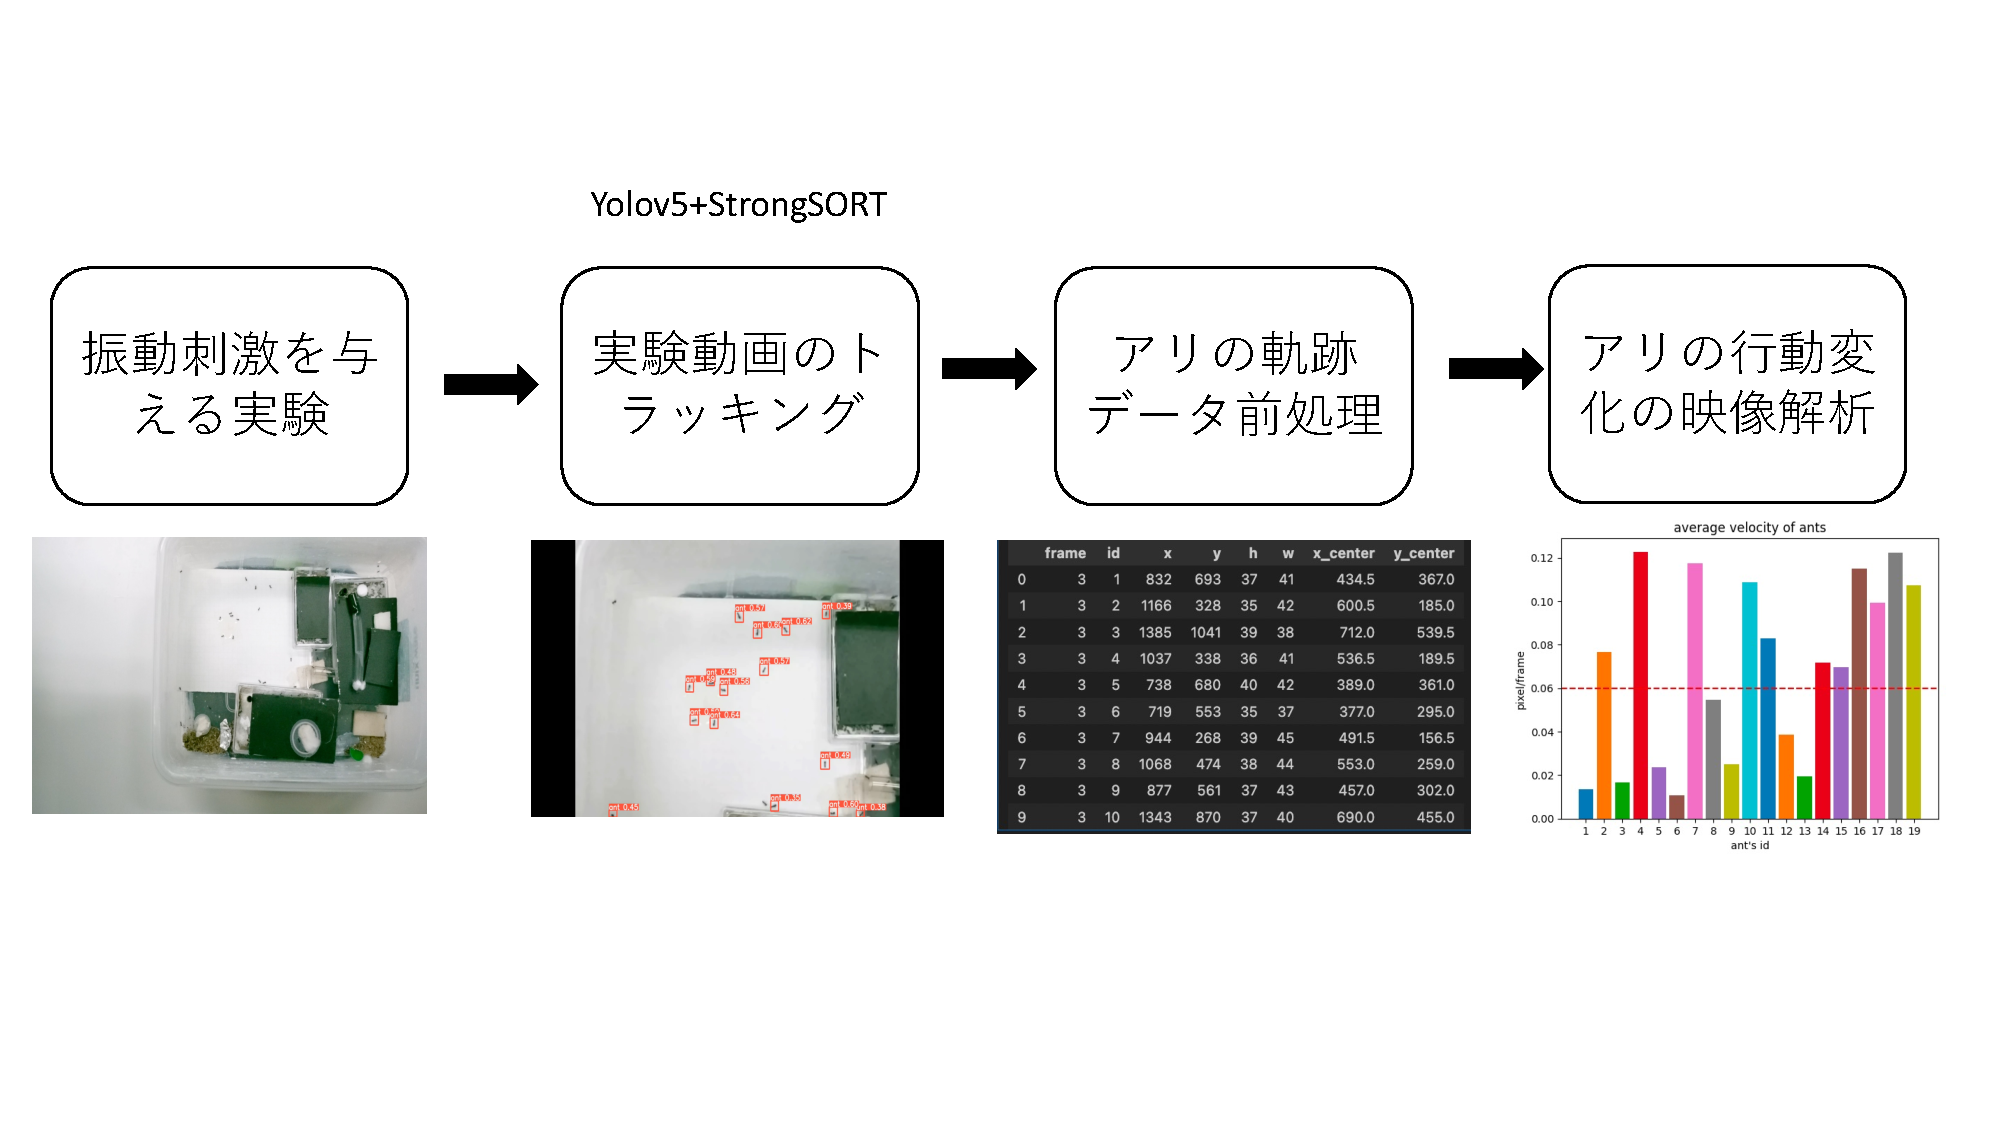
\includegraphics[width=\linewidth]{nagare.pdf}
\caption[Short figure caption for List of Figures]{提案手法全体図}
\label{fig:paper1_fig1}
\end{figure}

\section{軌跡データを用いたアリの行動解析}
追跡データ前処理を行った後,  解析を行う. まず全時間帯(全フレーム間)での平均速度を算出する. 結果からは,刺激を与えられると集団全体速度が上昇するが,その速度上昇期間は短く大体2秒間であり,その後集団全体はほぼ刺激前と同じ速度で動く. 次に, それぞれの個体平均速度を算出することで同じ刺激を与えられても「動かない」と「よく動く」アリがいることがわかった. そこでこの2つのグループの詳細行動変化を解析する. 

「動かない」アリの特徴は速度上昇期間が短く, 実験版の中心部またはコロニー(巣)の近くにいることである. 「よく動く」アリの特徴は速度上昇期間が集団全体と同じ期間でコロニーの向きに逃げる傾向があることである. さらに,「動かない」アリの方がうまく追跡でき,「よく動く」アリは移動速度が速いことが原因でうまく追跡できないことがあることも確認できた.

\section{おわりに}
本研究では,振動刺激に対するアリの行動変化を,映像からの個体追跡を行って解析した.実験や追跡手法の改善は必要であり,精度は不十分であるものの,映像データからアリの集団としての動きを解析する枠組みを構築し,特徴的なアリの行動変化を確認することができた.

{ 
\small
\begin{thebibliography}{99}

\bibitem{paper1}
林 叔克, 結城 麻衣. 少数の働きアリによる行動解析とモデル化. 計測自動制御学会東北支部 第247研究集会, 2008.

\bibitem{paper2}
白石允梓. アリの行動観察とその統計解析. 物性研究電子版, Vol.8, No.1, 2020



\end{thebibliography}
}

\end{document}
